\documentclass[a4paper,11pt]{article}
\usepackage[left=2.5cm, right=2.5cm, top=1.5cm, bottom=1.5cm]{geometry}
\usepackage{graphicx}
\usepackage{amssymb}
\usepackage{amsmath}
\usepackage[procnames]{listings}
\usepackage{xcolor}
\usepackage{hyperref}
\usepackage{enumerate}

\hypersetup{ %color attributes of citation, link, etc.
    colorlinks=true,
    linkcolor=blue,
    filecolor=gray,
    urlcolor=blue,
    citecolor=blue,
}

\setlength{\parindent}{0pt}

\newcommand\Item[1][]{%
  \ifx\relax#1\relax  \item \else \item[#1] \fi
  \abovedisplayskip=0pt\abovedisplayshortskip=0pt~\vspace*{-\baselineskip}}

%'codify' text for snippets
\usepackage{xcolor}
\definecolor{codegray}{gray}{1}
\newcommand{\code}[1]{\colorbox{codegray}{\texttt{#1}}}

\definecolor{keywords}{RGB}{255,0,90}
\definecolor{comments}{RGB}{0,0,113}
\definecolor{p_red}{RGB}{160,0,0}
\definecolor{p_green}{RGB}{0,150,0} 
\lstset{language=Python, 
        basicstyle=\ttfamily\small, 
        keywordstyle=\color{keywords},
        commentstyle=\color{comments},
        stringstyle=\color{p_red},
        showstringspaces=false,
        identifierstyle=\color{p_green},
		procnamekeys={def,class}}

\graphicspath{ {./images/} }
           
\begin{document}
\title{\LARGE{\textbf{ECEN405 Assignment 2}}}
\author{Niels Clayton : 300437590}
\date{}
\maketitle
\hrule

\subsubsection*{Q1}

\textit{In a single-phase diode rectifier bridge $I_s = 10$A(rms), $I_{s1}=8$A(rms) and DPF = 0.85}\\
\textbf{Calculate:} $I_{distortion}, \%THD, PF$

\begin{align*}
    I_{dist} & = \sqrt{I_{s}^{2}-I_{s1}^{2}}     \\
             & = 6A                              \\\\
    \%THD    & = 100\cdot\frac{I_{dist}}{I_{s1}} \\
             & = 75\%                            \\\\
    PF       & = \frac{I_{s1}}{I_{s}}DPF         \\
             & = 0.68
\end{align*}


\subsubsection*{Q2}
\textit{Calculate the percentage \textbf{harmonic distortion} of individual component and total THD for an output signal having a fundamental amplitude of 5V, second harmonic amplitude of 0.5V and a third and fourth harmonic components of 0.3 and 0.2.}\\

\begin{align*}
    HD_{2^{nd}} & = \frac{0.5}{5} = 10\%                                                \\\\
    HD_{3^{rd}} & = \frac{0.3}{5} = 6\%                                                 \\\\
    HD_{4^{th}} & = \frac{0.2}{5} = 4\%                                                 \\\\
    THD         & = \frac{\sqrt{ \sum_{n=2}^{\infty} \; V^2_{n\_rms} }}{ V_{fund\_rms}} \\\\
                & = \frac{\sqrt{ 0.5^2 + 0.3^2 + 0.2^2 }}{ 5 }                          \\
                & = 12.32\%
\end{align*}

\newpage
\subsubsection*{Q3}
\textit{A \textbf{magnetic core} has the following properties: The core Area $A_m = $ 0.931 cm$^2$, the magnetic path length is 3.76cm and the relative permeability of the material $\mu_r = $ 5000 }

\begin{enumerate}[i.]
    \item \textit{Calculate the Reluctance of the core.}

          \begin{align*}
              \mathfrak{R} & = \frac{l}{\mu_{r}\mu_{0}A}                                          \\
                           & = \frac{0.0376}{5000 \cdot 4\pi\times10^{-7}\cdot0.931\times10^{-6}} \\
                           & = 64277.4\;\;\;\mathrm{ampere \; turns/Wb}
          \end{align*}


    \item \textit{Calculate the reluctance of an air gap of length 1mm is introduced in the core.}
    
    \begin{align*}
        \mathfrak{R}_{core} &= \frac{0.0376 - 0.001}{5000\cdot 4\pi\times10^{-7}\cdot 0.931\times 10^{-6}} \\
        &= 62567.9 \;\;\;\mathrm{ampere \; turns/Wb}\\\\
        \mathfrak{R}_{air} &= \frac{0.001}{1\cdot 4\pi\times10^{-7}\cdot 9.31\times 10^{-5}} \\
        &= 8547526.48 \;\;\;\mathrm{ampere \; turns/Wb}\\\\
        \mathfrak{R} &= \mathfrak{R}_{core} +\mathfrak{R}_{air} = 62567.9 + 8547526.48\\
        &= 8611803.8 \;\;\;\mathrm{ampere \; turns/Wb}
    \end{align*}



    \item \textit{A coil with 25 turns is wound on the core with an air gap introduced in ii. Calculate the inductance of the coil.}

    \begin{align*}
        L &= \frac{N^2}{\mathfrak{R}} = \frac{25^2}{8.611\times 10^6}\\
        &= 7.258\times 10^{-5}H = 72.58\mu H
    \end{align*}

    \item \textit{If the flux density in the core of question (iii) is not to exceed 0.2T, what is the maximum current that can be allowed to flow through the inductor coil?}
    
    $$ B = \frac{\Phi}{A}, \hspace{2mm} \Phi = \frac{N \cdot i}{\mathfrak{R}} \rightarrow B = \frac{N \cdot i}{\mathfrak{R} \cdot A} $$
    \begin{align*}
        i&= \frac{B \cdot \mathfrak{R} \cdot A}{N}\\
        &= \frac{0.2\cdot 8.611\times10^6\cdot 9.31\times 10^{-5}}{25} = 6.41A
    \end{align*}


    \item \textit{At the maximum current calculated in question (iv), calculate the energy stored in the magnetic core and the air gap. Compare the two.}\\
    

    Volume of Air Gap:
    $$V = 9.31\times10^{-5}\cdot 10^{-3} = 9.31\times10^{-8}m^3$$

    Energy in Air Gap:
    \begin{align*}
        E &= \frac{1}{2}\cdot \frac{B^2}{\mu_0 \mu_r}\cdot V = \frac{1}{2} \cdot\frac{0.2^2}{4\pi\times10^{-7}\cdot 1}\cdot 9.31\times10^{-8}\\
        &= 1.482\times 10^{-3}J
    \end{align*}


    Volume of Core:
    $$V = 9.31\times10^{-5}\cdot 3.76^{-2} = 3.5\times10^{-6}m^3$$

    Energy in Core:
    \begin{align*}
        E &= \frac{1}{2}\cdot \frac{B^2}{\mu_0 \mu_r}\cdot V = \frac{1}{2}\cdot\frac{0.2^2}{4\pi\times10^{-7}\cdot 5000}\cdot 3.5\times10^{-6}\\
        &= 1.11\times 10^{-5}J
    \end{align*}

    There is 133.5 times as much energy stored in the air gap as there is stored in the magnetic core. \\

\end{enumerate}


\subsubsection*{Q4}
\textit{A current of 50mA is applied to the coil of example in \textbf{EM} lecture slide 17 (replicated below). Find the total flux ($\Phi$) in the core, the flux density B, and the magnetic field intensity H.}

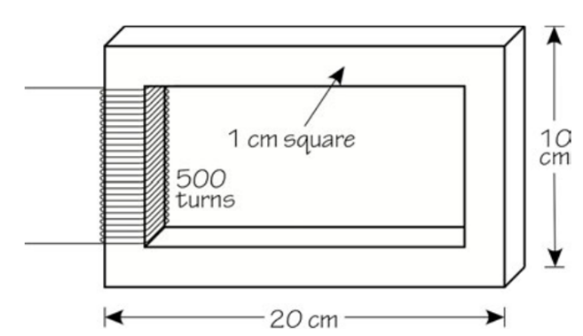
\includegraphics[width=0.5\textwidth]{core.png}

\begin{align*}
    \Phi & = \frac{L\cdot i}{n} = \frac{50.5\times10^{-3} \cdot 50 \times 10^{-3}}{500}                           \\&= 5.05\times10^{-6}\;\;Wb\\\\
    B    & = \frac{\Phi}{A} = \frac{5.05\times10^{-6}}{10^{-4}}                                                   \\
         & = 5.05\times10^{-3} \;\;T                                                                              \\\\
    H    & = \frac{B}{\mu} = \frac{B}{\mu_r \cdot \mu_0} = \frac{5.05\times10^{-3}}{900 \cdot 4\pi\times 10^{-7}} \\
         & = 4.465 \;\;\;\mathrm{ampere \; turns/m}                                                               \\\\
\end{align*}



\subsubsection*{Q5}
\textit{For a similar \textbf{motor} discussed in an example in the lecture notes, the rated efficiency was 91.7\%. Catalogue data shows voltage is 230/460 V, current is 25/12.5 A and power factor is 82\%, full-load speed is 1765 rpm. Check (write your procedure) the efficiency is correct with the given data. How much will it cost to run the motor at full load for 16 hours per day, five days a week, and 50 weeks a year? Assume the plant has a contracted rate of 12 cents per kwh.}

\begin{align*}
    P_{in} & =\sqrt{3}\times460\times12.5\times0.82 \\
           & = 8.167kW \\
    P_{out} &= 10(746) = 7.46kW \\
    \%\eta &= 100(7.46/8.167)=91.343\%
\end{align*}


\subsubsection*{Q6}

\textit{A 10-hp, 3-phase, 50-Hz \textbf{motor} has a full-load speed of 1,165 rpm. It is rated at 230/460 volts, 34.0/17.0 amperes full load, 71\% power factor. Rotational losses are estimated to be 175 W. Find the following:}

\begin{enumerate}[a)]
    \item \textit{Number of poles and slip:}\\
    \begin{align*}
        p &= \frac{2\cdot 60 \cdot f}{n_s} = \frac{6000}{1165}\\
        &\approx 5
    \end{align*}
    5 pole pairs gives the closest above 1165
    \begin{align*}
        n_{s(p=5)}&\rightarrow1200 \\
        \mathrm{Slip:\;s}&=100(1200-1165)/1200=2.9167\%
    \end{align*}

    \item \textit{Torque output:}\\
    \begin{align*}
        \omega_m &= (1165/50)2\pi = 146.39822 \mathrm{rad/s} \\
        T_{out} &= P_{out}/\omega_m \\
        &= 10(746)/146.39822=7460/146.39822
        \\&=50.96Nm
    \end{align*}

    \item \textit{Power input and efficiency:}\\
    \begin{align*}
        P_{in} &= \sqrt{3}\times460\times17\times0.71\\
        &=9616.6925W\\
        \%\eta &= 100(7460/9616.6925)=77.57\%
    \end{align*}

    \item \textit{Power lost in the rotor and stator:}\\
    \begin{align*}
        P_{devel} &= 7460+175=7635W\\ 
        P_{airgap} &= 7635/(1-0.029167)=7864.38W \\
        P_{rotor} &= P_{airgap}-P_{devel} = 7864.38-7635=229.38W \\
        P_{stator} &= 9616.69-7864.38=1752.31W
    \end{align*}
\end{enumerate}


\subsubsection*{Q7}
\textit{For the above motor, specify the capacitance per phase (in kVARs) needed to improve the power factor to 92\%. Then find the magnitude of the line current with the added capacitance}



\subsubsection*{Q8}
\textit{In a single phase 50Hz \textbf{power factor correction} circuit, $V_s$ = 240V (rms), $V_d$ = 500V and the output power is 600W. Calculate $i_L(t)$, $d(t)$ and the average current $i_d$ through the output diode. Calculate the second harmonic peak voltage in the capacitor if C = 690$\mu$F}



\subsubsection*{Q9}
\textit{In a 2-pole, three-phase \textbf{PMAC motor drive}, the torque constant $k_{T(\phi)}$ and the voltage constant $k_{E(\phi)}$ are 0.5 in MKS units. The synchronous inductance is 20mH (neglect the winding resistance). This motor is supplying a torque of 3 Nm at a speed of 3,000 rpm in a balanced sinusoidal steady state. Calculate the per-phase voltage across the power-processing unit as it supplies controlled currents to this motor.}



\end{document}